
Figure~\ref{fig:calib-FTmap} shows the current cryostat design for the %DUNE SP FD 
\dword{spmod} with penetrations for various subsystems. The penetrations dedicated to calibration are the highlighted black circles. 

In addition to these dedicated ports, there are plans to use the \dword{dss} and cryogenics ports (orange and blue dots in Figure~\ref{fig:calib-FTmap}) as needed to route cables for other calibration systems, e.g., fiber optic cables for the \dword{pd} calibration system, which is described in Chapter~\ref{ch:fdsp-pd}. \dword{dss} and cryogenics ports can be accommodated by feedthroughs with a CF63 side flange for this purpose.   

\begin{dunefigure}[Cryostat penetration map with calibration ports]{fig:calib-FTmap}
{Top view of the \spmod %DUNE SP FD 
cryostat showing various penetrations. Circles highlighted in black are multi-purpose calibration penetrations. The green dots are \dword{tpc} signal cable penetrations. The blue ports are cryogenics ports. The orange ports are \dword{dss} penetrations. The larger purple ports at the four corners of the cryostat are human access ports.}
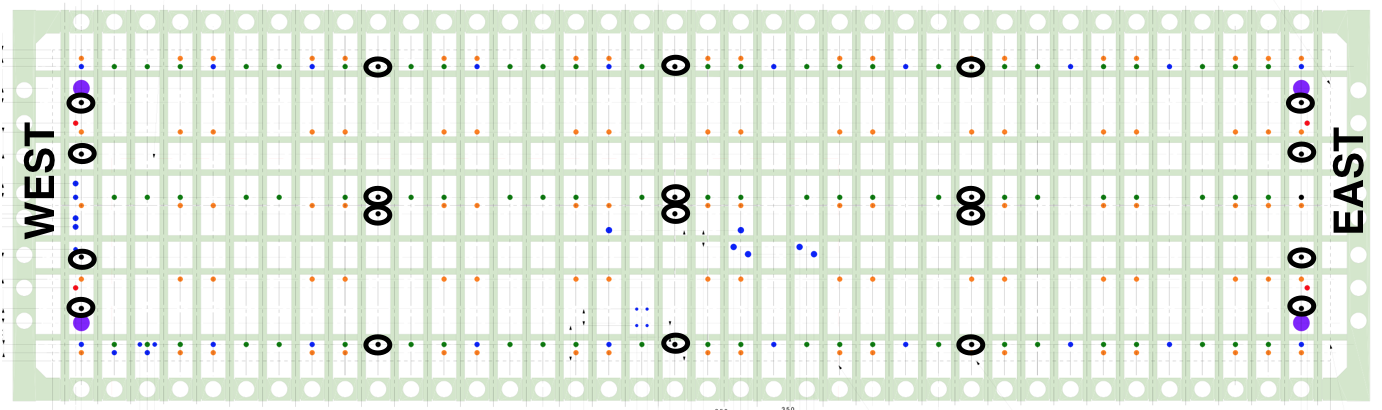
\includegraphics[height=2.0in]{calib-FTmap.png}
\end{dunefigure}

The current plan is to use the calibration ports for several different purposes, but their placement is largely driven by requirements for the ionization track laser. %and radioactive source system. 
The ports %that are %inwards 
toward the center of the cryostat are placed near the \dword{apa}s, where the \efield is small, %\fixme{check} 
to minimize any risks due to %the
\dword{hv} discharge. \dword{hv} is not an issue for the far east and west ports since they are located outside the \dword{fc} and the penetrations are located %near 
close to mid-drift (a location favorable for possible source deployment).
%to meet radioactive source requirements. 
%\fixme{The amendment above may need some work. I won't look at it until it's ready.}
Implementing the baseline ionization track laser system as %proposed 
described in Section~\ref{sec:sp-calib-sys-las-ion} requires \num{12} feedthroughs, the three central ones in each of the four \dword{tpc} drift volumes; this arrangement allows lasers to be used for full volume calibration of the \efield and associated diagnostics (e.g., \dword{hv}). 

The distance between any two consecutive feedthrough columns shown in Figure~\ref{fig:calib-FTmap} is approximately \SI{15}{\m}. Since the \dword{microboone} laser system has shown that tracks will propagate over that detector's full \SI{10}{\m} length, this distance is considered reasonable. Assuming that the effects of Rayleigh scattering and self-focusing (Kerr effect) do not limit the laser track length, this laser arrangement could illuminate the full volume with crossing tracks in the central region, and single tracks %coverage 
in the region closer to the end-walls.  %Please note that, 
At this time, the maximum usable track length is unknown, and it may be that the full \SI{60}{\m} \detmodule length could be covered by the laser system after optimization.

Throughout this chapter, the following convention for the coordinate axes will be used: $x$ is parallel to the drift direction, $y$ is the vertical, and $z$ is parallel to the beamline. This is illustrated in Chapter~\ref{ch:sp-cisc} Figure~\ref{fig:cfd-example-geometry}.
